\documentclass{article}
\usepackage{amssymb} %math
\usepackage{amsmath} %math
\usepackage{cmap} %ability to copy russian
\usepackage[T2A]{fontenc} %encoding for babel
\usepackage[russian]{babel} %russian
\usepackage{amsthm} %theorems
\usepackage{imakeidx} %indexing
\usepackage{fancyhdr}
\usepackage{color}
\usepackage{graphicx} %images
\usepackage{hyperref} %hyperlinks
\hfuzz=30pt
\vfuzz=30pt
\hbadness=2000


\pagestyle{fancy}
\makeindex[title=Указатель, intoc, options=-s indexstyle.ist]

\fancyhead{}
\fancyhead[LO]{\hyperlink{t1}{к содержанию}}
\fancyhead[CO]{\hyperlink{t2}{к указателю}}

\hypersetup{
     colorlinks=true,
     linkcolor=magenta,
     filecolor=red,
     citecolor=red,      
     urlcolor=blue,
}

\title{\hypertarget{t1}{Билеты по матанализу за второй семестр}}
\author{}
\date{}

\newtheoremstyle{indented}{0 pt}{0 pt}{\itshape}{}{\bfseries}{. }{0 em}{ }
\theoremstyle{indented}
\newtheorem{theorem}{Теорема}
\newtheorem{lemma}{Лемма}
\newtheorem{stat}{Утверждение}

\theoremstyle{definition} 
\newtheorem{defn}{Определение}
\newtheorem*{exl}{Пример(ы)}


\theoremstyle{remark} 
\newtheorem*{remark}{Примечание}
\newtheorem*{remind}{Напоминание}
\newtheorem*{cons}{Следствие}
\newtheorem*{exer}{Упражнение}

\newcommand{\htarg}[2]{\hypertarget{#1}{\textcolor{magenta}{#2}}}
\newcommand{\hlink}[2]{\hyperlink{#1}{#2}}
\newcommand{\hindex}[2]{\index{#2@\protect\hyperlink{#1}{#2}}}
\newcommand{\add}[2]
{
    \hypertarget{#1}{\textcolor{magenta}{#2}}
    \index{#2@\protect\hyperlink{#1}{#2}}
}
\newcommand{\df}[2]{\frac{\delta #1}{\delta #2}}

\begin{document}


\maketitle
\tableofcontents

\newpage

%1, примеры?
\section{Функции ограниченной вариации. Свойства. Замена переменной. Примеры.}


\begin{defn}
    \add{var}{Вариация функции}
    $f: \mathbb{R} \to \mathbb{R}^m$
    \[
        V_f([a,b])=\sup\limits_{
            \begin{smallmatrix}
                x_0 \leq x_1 \leq \dots \leq x_n \\
                x_0=a, x_n=b
            \end{smallmatrix}
        }
        \sum\limits_{k=0}^{n-1} |f(x_{k+1})-f(x_k)|
    \]
\end{defn}

\begin{remark}
    Свойства вариации
    \begin{itemize}
        \item $f: \mathbb{R}\to\mathbb{R}, f$ монотонна $\Rightarrow V_f([a,b])=|f(a)-f(b)|$
        \item $V_f([a,b])=0 \Leftrightarrow f$ константо на $[a,b]$
        \item $V_{f+g} \leq V_f + V_g$
        \item $V_f$ аддитивна по промежутку: \\ $a\leq b\leq c: V_f([a,c])=V_f([a,b])+V_f([b,c])$
    \end{itemize}
\end{remark}

\begin{remark}\hindex{bound var}{Ограниченная вариация}
    Будем говорить, что $f$ имеет \htarg{bound var}{ограниченную вариацию}
    на $[a,b]$, если $V_f$ конечна на $[a,b]$
\end{remark}

\begin{stat}
    Для $f: \mathbb{R}\to\mathbb{R}$ следующие утверждения эквивалентны
    \begin{enumerate}
        \item $f$ имеет ограниченную вариацию на $[a,b]$
        \item $f=f_1-f_2$, для каких-то  $f_1, f_2$ неубывающих на $[a,b]$
    \end{enumerate}
\end{stat}

\begin{proof}
    "$1\rightarrow2$": рассмотрим $\phi(x) = V_f([a,x]) \Rightarrow \phi \nearrow$\\
    $f = \phi - (\phi-f)$, пусть $h=\phi-f$. $h\nearrow \Leftrightarrow$ при $x\leq y$:
    $h(x)\leq h(y) \Leftrightarrow \phi(x)-f(x) \leq \phi(y)-f(y) \Leftrightarrow f(y)-f(x) \leq \phi(y) - \phi(x) = V_f([x,y])$\\
    "$2\rightarrow1$": $V_{f_1-f_2}[a,b] \leq V_{f_1}[a,b] + V_{-f_2}[a,b] = |f_1(a)-f_1(b)|+|f_2(a)-f_2(b)|$
\end{proof}

\begin{stat}
    (\add{replace var}{Замена переменной в вариации})
    Пусть $g: [a,b] \to [c,d]$ непрерывная биекция,
    тогда $V_f[c,d]=V_{f\circ g}[a,b]$
\end{stat}

\begin{proof}
    $g$ монотонна, будем считать, что возрастает. Любому набору $x_0, x_1, \dots, x_n$ из определения вариации $V_f$ найдутся соответсвующие  $y_0, y_1, \dots, y_n$,
    удовлетворяющие условию $g(y_k)=x_k$ и подходящие для подстановки в определение $V_{f\circ g}$, т.к. $y_k \nearrow \Leftrightarrow g(y_k) \nearrow$. Тогда $V_f[c,d]\leq V_{f\circ g}[a,b]$,
    но с другой стороны $V_f[c,d]\geq V_{f\circ g}[a,b]$, т.к. можно подставлять $x_k:=g(y_k)$ в определение первой вариации.
\end{proof}

%2
\section{Естественная параметризация. Гладкие пути. Длина гладкого пути.}


\hindex{curve}{Кривая}
\begin{defn}
    Множество в $\mathbb{R}^n$ называют \htarg{curve}{кривой}, если оно является образом некоторой непрерывной функции $f: (a,b)\to \mathbb{R}^n$.
    Дуга кривой (или же путь) - подмножество кривой $f: [c,d] \to \mathbb{R}^n$.
\end{defn}

\hindex{lenc}{Длина кривой (пути)}
\begin{defn}
    \htarg{lenc}{Длина дуги кривой (пути)} $f: [a,b]\to \mathbb{R}^n$ это $V_f([a,b])$.
\end{defn}

\begin{remark}
    Если длина пути конечна, то путь называется спрямляемым, иначе - неспрямляемым.
\end{remark}

\begin{defn}
    Естественная параметризация кривой - параметризация длиной её дуги, отсчитываемой от фиксированной точки.
\end{defn}

\begin{remark}
    Естественная параметризация - параметризация, которая "равномерна по времени, т.е. за одинаковый промежуток времени проходим одинаковое расстояние".
\end{remark}

\subsection*{Естественная параметризация спрямляемого пути}

$\phi:[a,b]\to[0,\beta], \phi(x)=V_f([a,x])$, если $\phi$ строго возрастает (путь $"$без остановок$"$, $f\not\equiv const$ ни на каком интервале),
то $\phi$ - биекция и \\
$\exists \psi: [0,\beta]\to[a,b], \psi=\phi^{-1}, V_f([a,b])=\phi(b)-\phi(a)$\\
$V_{f\circ \psi}([c,d])=V_f([\psi(c),\psi(d)]) = \phi(\psi(d))-\phi(\psi(c))=d-c$

\begin{defn}
    \add{smoothc}{Гладкий путь} - образ гладкой $f: [a,b] \to \mathbb{R}^n$ (т.е. $f=(f_1,...,f_n)$, причём все $f_k$ непрерывно дифференцируемы).
\end{defn}

\begin{remind}
    \htarg{lagrange}{Формула Лагранжа}, $f: [a,b] \to \mathbb{R}$ дифференцируема $\Rightarrow \exists \xi \in (a,b):$
    $$f'(\xi) = \frac{f(a)-f(b)}{a-b}$$
\end{remind}

\begin{stat}
    \add{lensmoothc}{Длина гладкого пути} 
    $f=(f_1, ..., f_n)$ равна $\displaystyle \int_{a}^{b}{\sqrt{\sum\limits_{m=1}^{n}(f'_m(x))^2}} dx$
\end{stat}

\begin{proof}
    Рассмотрим $V_f([a,b]) = \displaystyle \sup_{x_0=a, ..., x_N = b} \sum\limits_{k=0}^{N-1} |f(x_{k+1})-f(x)|$ и 
    воспользуемся формулой Лагранжа $\sum\limits_{k=0}^{N-1} \sqrt{\sum\limits_{m=1}^{n}(f_m(x_{k+1})-f_m(x_k))^2} = \\$
    $\sum\limits_{k=0}^{N-1} (x_{k+1}-x_k) \sqrt{\sum\limits_{m=1}^{n} (f'_m(\xi_{m,k}))^2}=(V),$
    $\ \xi_{m,k} \in (x_k,x_{k+1}), (f'_m)^2$ равномерно непрерывна на $[x_k, x_{k+1}]$, значит для любого $\varepsilon > 0$ 
    существует достаточно малое разбиение $[a,b]$ такое, что 
    $(f'_m)^2(\xi_{m,k}) \leq \min_{[x_k, x_{k+1}]} (f'_m)^2 + \varepsilon^2$ . Тогда
    \[  (I) \leq (V) \leq \underbrace{\sum\limits_{k=0}^{N-1} (x_{k+1}-x_k) \sqrt{\sum\limits_{m=1}^{n} \min_{[x_k, x_{k+1}]} (f'_m)^2}}_{(I)} 
    +  \varepsilon \sqrt{n} \cdot \underbrace{(b-a)}_{\sum\limits_{k=0}^{N-1} (x_{k+1}-x_k)} \]
    Левая и правая части стремятся к интегралу из условия (при стремлении 
    мелкости к нулю), тогда по \href{https://ru.wikipedia.org/wiki/%D0%A2%D0%B5%D0%BE%D1%80%D0%B5%D0%BC%D0%B0_%D0%BE_%D0%B4%D0%B2%D1%83%D1%85_%D0%BC%D0%B8%D0%BB%D0%B8%D1%86%D0%B8%D0%BE%D0%BD%D0%B5%D1%80%D0%B0%D1%85}
    {теореме о двух миллиционерах} туда же стремится и $(V)$.
\end{proof}

\subsection*{Естественная параметризация гладкого пути}

$\displaystyle \phi(x)=V_f([a,x])=\int_{a}^{x} |f'(t)| dt = \int_{a}^{x}{\sqrt{\sum\limits_{k=1}^{n}(f'_k(t))^2}} dt$\\
Параметризация всё также по длине дуги $\psi = \phi^{-1}$
\begin{stat}
    $|(f(\psi(x)))'|=1$
\end{stat}

\begin{proof}
    $\phi'(x)=|f'(x)|, \psi'(x)=\frac{1}{\phi'(\psi(x))}=\frac{1}{|f'(\psi(x))|}$\\
    $|(f(\psi(x)))'|=|f'(\psi(x))\cdot\psi'(x)|=1$
\end{proof}

%3
\section{Движение по окружности. Единственность простого вращения.}


Единичная окружность описывается уравнением $x^2+y^2=1$.
Хотим обойти её с единичной скоростью, начиная с точки (1,0).

Комплексные обозначения: рассмотрим биекцию $\mathbb{R}^2$ с $\mathbb{C}$ по правилу:
$(x,y) \leftrightarrow (x+iy)$. Тогда путь можно рассматривать как отображение из $\mathbb{R}$ в $\mathbb{C}$.

\begin{defn}
    \add{rotation}{Простое вращение}
    по окружности это отображение \\
    $\Gamma: \mathbb{R} \to \pi=\{ z\in \mathbb{C} \big| |z| = 1 \} = \{ z\in \mathbb{C} \big| x,y\in \mathbb{R}, x^2+y^2=1, z=x+iy \}$,
    \begin{itemize}
        \item $\Gamma \in C^1$ (гладкая)
        \item $\Gamma(0)=1, \Gamma'(0)=i$
        \item $|\Gamma'(t)|=1$ для любого $t$
    \end{itemize}
\end{defn}

\begin{lemma}
    $\Gamma'(t)\equiv i\Gamma(t)$
\end{lemma}

\begin{proof}
    $\Gamma(t)\in\pi \Rightarrow |\Gamma(t)|=\Gamma(t)\overline{\Gamma(t)} = 1$\\
    $\Rightarrow (\Gamma(t)\overline{\Gamma(t)})' = \Gamma'(t)\overline{\Gamma(t)}+\Gamma(t)\overline{\Gamma'(t)} = 0$\\
    $\Rightarrow 2\Re(\Gamma'(t)\overline{\Gamma(t)})= 0,$
    $|\Gamma'(t)|=|\overline{\Gamma(t)}|=1$ и $\Gamma'(0)\overline{\Gamma(0)}=i$
    $\Rightarrow \Gamma'(t)\overline{\Gamma(t)} \equiv i$
\end{proof}

\begin{stat}
    Если $\Gamma$ существует, то оно единственно.
\end{stat}

\begin{proof}
    Пусть $\Gamma_1, \Gamma_2$ - простые вращения, тогда по лемме\\
    $(\Gamma_1 \overline{\Gamma_2})'=\Gamma_1' \overline{\Gamma_2}+\Gamma_1 \overline{\Gamma_2'}$
    $= i \Gamma_1 \overline{\Gamma_2} + \Gamma_1 \overline{i\Gamma_2} = 0$
    $\Rightarrow \Gamma_1 \overline{\Gamma_2} = const, \Gamma_1(0) \overline{\Gamma_2(0)}=1$\\
    $\displaystyle \Rightarrow \Gamma_1 \overline{\Gamma_2} = 1 \Rightarrow \Gamma_1 = \frac{1}{\overline{\Gamma_2}} = \frac{\Gamma_2}{|\Gamma_2|} = \Gamma_2$
\end{proof}

%4, функции? свойства? формула Эйлера?
\section{Построения простого вращения. Тригонометрические функции. Свойства. Формула Эйлера.}


\begin{stat}
    \hlink{rotation}{Простое вращение} $\Gamma(t)$ существует.
\end{stat}
%доделать
\begin{proof}
    $\pi=\{  z=x+iy \big| x,y\in \mathbb{R}, x^2+y^2=1 \}$\\
    $-1 \leq t \leq 1: x = t, \ y = \sqrt{1-t^2}$\\
    $1 \leq t \leq 3: \ x = 2-t, \ y = -\sqrt{1-(2-t)^2}$\\
    Покажем, что после естественной параметризации есть гладкость и `на краях`,
    $f_1'(t)=1, f_2'(t)=-\frac{t}{\sqrt{1-t^2}}$\\
    $\phi (x) = \int_{-1}^x |f'(t)| dt = \int_{-1}^x \sqrt{1+\frac{t^2}{1-t^2}} dt = \int_{-1}^{x} 
    \frac{1}{\sqrt{1-t^2}} dt$ этот интеграл сходится, т.к. особенность порядка $\frac{1}{2}$.
    \textit{Пояснение:} из первого семестра мы знаем, что 
    $\int_{0}^{1} \frac{dt}{t^\alpha} $ сходится $\Leftrightarrow  \alpha < 1$, а в данном случае 
    достаточно рассмотреть $\int_0^1 \frac{dt}{\sqrt{1-t^2}} = \int_0^1 \frac{dt}{\sqrt{1-t}\sqrt{1+t}} $,
    он сходится, т.к. $\int_0^1 \frac{dt}{\sqrt{1-t}} = \int_0^1 \frac{dt}{\sqrt{t}}$ сходится и можно, например,
    применить признак Абеля, чтобы домножить аргумент на $\frac{1}{\sqrt{1+t}}$.
\end{proof}

%5 примеры?
\section{Дифференцируемость отображений между евклидовыми пространствами. Свойства. Примеры.}


\begin{defn}
    \add{norma}{Норма} на евклидовых пространствах - отображение из $\mathbb{R}^n$ в $\mathbb{R}_+$, удовлетворяющее условиям:
    \begin{enumerate}
        \item $||x||=0 \Leftrightarrow x=0$
        \item $||\alpha x|| = |\alpha| \cdot ||x||, \forall \alpha \in \mathbb{R}$
        \item $||x+y|| \leq ||x|| + ||y||$
    \end{enumerate} 
\end{defn}

\begin{remark}
    Все расстояния мы будем рассматривать с евклидовой нормой
    (т.е. $d(x,y)=||x-y||=\sqrt{\sum\limits_{k=1}^{n}(x_k-y_k)^2}$).
    Такая метрика стандартна. Так как в этом семестре рассматриваемые размерности 
    евлидовых пространств конечные, то с точки зрения сходимостей к нулю мы можем считать 
    разные нормы эквивалентными.
\end{remark}

\begin{remind}
    \htarg{modv}{Модуль (или длина) евклидова вектора} $x=(x_1,x_2, ... , x_n)$:
    \[
        |x|=\sqrt{\sum\limits_{k=1}^{n}x_k^2}
    \]
\end{remind}

\hindex{dif}{Дифференциал}
\hindex{der}{Производная}
\begin{defn}
    $f: \mathbb{R}^n \to \mathbb{R}^m$ дифференцируема в точке $a$, если
    существует линейное отображение $L$, такое что $f(x)=f(a)+L(x-a)+o(||x-a||)$,
    $L$ называют \htarg{der}{дифференциалом} функции $f$ в точке $a$.
    $L$ определяется матрицей $A$ размера $m \times n$, её столбцы -
    это значения на базисных векторах, $A$ называют \htarg{der}{производной} функции.
\end{defn}

\begin{remark}
    Запись $f(x)=f(a)+L(x-a)+o(||x-a||)$ означает, что
    \[ \forall \varepsilon > 0 \ \exists \delta: \ \ 0 < ||x-a|| < \delta \Rightarrow \frac{|f(x)-f(a)-L(x-a)|}{||x-a||} < \varepsilon \]
\end{remark}

\begin{remark}
    Если $L$ существует, то оно единственно.
    \begin{proof}
        Пусть $L_1$ и $L_2$ дифференциалы $f$ в точке $a$, тогда \\
        $(L_1-L_2)(x-a)=o(||x-a||)$ при $x\to a$, это возможно только
        если отображение $(L_1-L_2)$ тождественный нуль.\\
        \textit{Пояснение: } пусть $L(x)=o(||x||), x=(x_1,...,x_n)$; $L(x)=\sum\limits_{k=1}^{n} L(x_k e_k) =
        \sum\limits_{k=1}^{n} x_k L(e_k)$, где $e_k$ - базисные вектора. 
        Пусть $\exists k: L(e_k)\not=0 \Rightarrow $ для векторов вида $y=a e_k, a\in\mathbb{R}_{>0}, a \to 0$,
        $\frac{L(y)}{||y||}=\frac{aL(e_k)}{a||e_k||}=\frac{L(e_k)}{||e_k||} \not=0 $, противоречие. 
    \end{proof}
\end{remark}

%6
\section{Отделимость линейных отображений от нуля. Норма в пространстве линейных отображений.}


\begin{defn}
    \add{linnorma}{Норма линейного отображения} $L$:
    $$
        ||L|| = \sup_{||x|| \leq 1} ||Lx||
    $$
\end{defn}

\begin{remark}
    Следующие нормы эквивалентны: 
    \begin{itemize}
        \item $||L|| = \sup_{||x|| \leq 1} ||Lx||$
        \item $||L|| = \sup_{||x|| = 1} ||Lx||$
        \item $||L|| = \sup_{||x|| < 1} ||Lx||$
        \item $||L|| = \sup_{||x|| \not= 0} \frac{||Lx||}{||x||}$
    \end{itemize}
    $$$$
\end{remark}

\begin{stat}
    (Линейное отображение липшицево)
    $L: \mathbb{R}^n \to \mathbb{R}^m$ линейно, значит $\exists A: \ \forall x,y \in \mathbb{R}^n: \ ||Lx-Ly|| \leq A||x-y||$
\end{stat}

\begin{remark}
    $||L||=min\{A \big| \   \forall x,y \in \mathbb{R}^n: \ ||Lx-Ly|| \leq A||x-y||\}$
\end{remark}

%7
\section{Дифференцирование суммы, произведения, частного.}

%8
\section{Дифференцирование суперпозиции функций.}

%9
\section{Частные производные. Связь частных производных с дифференцируемостью. Производная по направлению.}


\hindex{partder}{Частная производная}
\begin{defn}
    \htarg{partder}{Частной производной}
    функции $f$ по $i$-ой координате в точке $A=(a_1, a_2, ..., a_n)$ называют предел:
    $$f'_{x_i}(A) = \frac{\delta f}{\delta x_i} (A) = \lim\limits_{x_i \to a_i} \frac{f(a_1, ..., a_{i-1}, x_i, a_{i+1}, ..., a_n) - f(a_1, ..., a_{i-1}, a_i, a_{i+1}, ..., a_n)}{x_i-a_i}$$
\end{defn}

\hindex{smooth}{Гладкость}
\begin{remark}
    Будем называть функцию \htarg{smooth}{гладкой}, если все её частные производные непрерывны.
\end{remark}

\begin{remind}
    Неравенство Коши-Буняковского-Шварца (КБШ):
    \[
        \left(\sum\limits_{k=1}^{n}x_k y_k\right)^2 \leq
        \left(\sum\limits_{k=1}^{n}x_k^2\right)
        \left(\sum\limits_{k=1}^{n}y_k^2\right)
    \]
\end{remind}

\begin{theorem}
    Если все частные производные $f: \mathbb{R}^n \to \mathbb{R}^m$ непрерывны в некоторой окрестности точки $x^0$, то $f$ дифференцируема в $x^0$.
\end{theorem}

\begin{proof}
    Рассмотрим случай $m=1$.
    $x^0 = (x_1^0,...,x_n^0)$.
    Применим \hlink{lagrange}{формулу Лагранжа} $f(x)-f(x^0)=f(x_1,...,x_n)-f(x_1^0,...,x_n^0)=$\\
    $\sum\limits_{k=1}^{n} \left(f(x_1^0,...,x_{k-1}^0,x_k,x_{k+1}...,x_n)-f(x_1^0,...,x_{k-1}^0,x_k^0,x_{k+1}...,x_n)\right)=$\\
    $\sum\limits_{k=1}^{n} f'_{x_k}\big|_{(x_1^0,...,x_{k-1}^0,\xi_k,x_{k+1},...,x_n)} (x_k-x_k^0)\overbrace{=}^? \sum\limits_{k=1}^{n} f'_{x_k}\big|_{x^0}(x_k-x_k^0) + o(|x-x^0|)$\\
    $\Leftrightarrow\sum\limits_{k=1}^{n} (f'_{x_k}\big|_{t_k} - f'_{x_k}\big|_{x^0}) (x_k-x_k^0)\overbrace{=}^? o(|x-x^0|)$, |LHS| оценивается по неравенству КБШ как
    $\sqrt{\sum\limits_{k=1}^{n} \left(f'_{x_k}\big|_{t_k} - f'_{x_k}\big|_{x^0}\right)^2} \cdot \sqrt{\sum\limits_{k=1}^{n} \left(x_k-x_k^0\right)^2} < \varepsilon \sqrt{n} \hyperlink{modv}{|x-x^0|}$
    при $|x-x_0| < \delta$ (пользуемся непрерывностью $f'_{x_k}$ в окрестности точки $x_0$ и тем, что $|t_k-x_0| < |x-x_0|$). Для $m>1$ достаточно представить $f$ в виде $f=(f_1,...,f_m)$ и рассмотреть каждую $f_k$ отдельно.
\end{proof}

\begin{remark}
    Наличия частных производных в точке недостаточно, чтобы сказать, что функция дифференцируема. 
\end{remark}

\begin{defn}
    \hindex{dirder}{Производная по направлению}
    \htarg{dirder}{Производной функции $f$ по направлению} единичного вектора $e$ в точке $x$ называется предел:
    \[
        \lim\limits_{
            \begin{smallmatrix}
                t\in \mathbb{R} \\
                t \to 0
            \end{smallmatrix}
        }
        \frac{f(x+te)-f(x)}{t}
    \]
\end{defn}

\begin{remark}
    Частная производная $f$ по $k$-ой координате это
    производная по направлению $(\underbrace{0,...,0}_{k-1}, 1, 0, ..., 0)$.
\end{remark}

\begin{remark}
    Производная $f(x_1,x_2,...,x_n)$ по направлению $e=(e_1, e_2, ..., e_n)$ выражается через частные производные $f$.
    \[
        f'_e(x)=\sum\limits_{k=1}^{n} e_k f'_{x_k}(x)
    \]
\end{remark}

%10
\section{Лемма о билипшицевости.}


%11 доказательство?
\section{Теорема об обратном отображении.}


\begin{theorem}
    Пусть $f: G \to \mathbb{R}^n (G -$ открытое в $\mathbb{R}^n)$.
    У $f$ есть частные непрерывные производные. $A$ - производная $f$
    в точке $x^0$, причём $A$ невырождена. Тогда в окрестности т. $x^0$
    существует гладкая $g$, т.ч. $g(f(x))=x$ и производная $g$ в т. $x^0$ это $A^{-1}$. 
\end{theorem}

\begin{stat}
    $f$ гладкая в окрестности $x^0$, значит она там же липшецева, т.е. $\exists C \ \forall x,y:\ |f(x)-f(y)| < C ||x-y||$
\end{stat}

\begin{stat}
    $Ker(A)=\{0\} \Rightarrow f$ билипшицева, т.е. $\exists C_1,\ C_2 > 0 \ \forall x,y: \ C_1||x-y|| < |f(x)-f(y)| < C_2 ||x-y||$
\end{stat}

%12 примеры?
\section{Матрица Якоби. Градиент.}


\begin{defn}
    \add{grad}{Градиент} это вектор, состоящий из частных производных $f: \mathbb{R}^n \to \mathbb{R}$
    \[
        \nabla f = \textrm{grad } f =
        \left(\frac{\delta f}{\delta x_1}, \frac{\delta f}{\delta x_2}, ... , \frac{\delta f}{\delta x_n} \right)
    \]
\end{defn}

\begin{remark} Свойства
    \begin{itemize}
        \item Градиент указывает направление вектора, вдоль которого функция имеет наибольшее возрастание
        \item $df = \sum\limits_{k}^{} \frac{\delta f}{\delta x_k} dx_k = \langle \textrm{grad } f, dx \rangle$
    \end{itemize}
\end{remark}

\begin{defn}
    \add{jacobi}{Матрица Якоби} - матрица состоящая из всех частных производных
    $f: \mathbb{R}^n \to \mathbb{R}^m, f=(f_1, f_2, ... , f_m)$
    \[
        J(x) =
        \begin{pmatrix}
            \frac{\delta f_1}{\delta x_1}(x) & \frac{\delta f_1}{\delta x_2}(x) & \dots  & \frac{\delta f_1}{\delta x_n}(x) \\
            \frac{\delta f_2}{\delta x_1}(x) & \frac{\delta f_2}{\delta x_2}(x) & \dots  & \frac{\delta f_2}{\delta x_n}(x) \\
            \vdots                           & \vdots                           & \ddots & \vdots                           \\
            \frac{\delta f_m}{\delta x_1}(x) & \frac{\delta f_m}{\delta x_2}(x) & \dots  & \frac{\delta f_m}{\delta x_n}(x) \\
        \end{pmatrix}
    \]
\end{defn}

\begin{remark} Свойства
    \begin{itemize}
        \item Строчки матрицы Якоби - градиенты соответствующих функций
        \item Если все $f_k$ непрерывно дифференцируемы в окрестности $a$, то матрица Якоби - производная $f$ в $a$,
              т.е. $f(x)=f(a)+J(a)(x-a)+o(|x-a|)$
        \item (Свойство функториальности) Если
              $\varphi: \mathbb{R}^n \to \mathbb{R}^m, \psi: \mathbb{R}^m \to \mathbb{R}^k$
              дифференцируемы, то $J_{\psi \circ \varphi}(x) = J_\psi(\varphi(x))J_\varphi(x)$
    \end{itemize}
\end{remark}

%13
\section{Дифференцирование обратного отображения.}

%14
\section{Теорема о равенстве смешанных производных.}
\begin{defn}
    \add{mixder}{Смешанная производная} порядка $k$ определяется индуктивно:\\
    \textit{База} $k=1$: обыкновенная \hyperlink{partial der}{частная производная} $\frac{\delta f}{\delta x_{i_1}}$\\
    \textit{Переход} $k\to k+1$: возьмём частную производную по $i_{k+1}$-ой координате в точке $A$ от частной производной порядка $k$, т.е.
    от $\frac{\delta^k f}{\delta x_{i_k}\delta x_{i_{k-1}}...\delta x_{i_1}}$ (должна быть определена в некоторой окрестности
    $A$), если соответствующий предел существует, то его и назовём смешанной частной производной порядка $k+1$, обозначим так:
    $\frac{\delta^{k+1} f}{\delta x_{i_{k+1}}\delta x_{i_k}...\delta x_{i_1}}$
\end{defn}

\begin{theorem}
    Пусть $f: G\subset \mathbb{R}^2 \to \mathbb{R}$ ($G$ открытое), $f=f(x,y)$,
    смешанные производные $\frac{\delta^2 f}{\delta x \delta y}$,
    $\frac{\delta^2 f}{\delta y \delta x}$ непрерывны в точке $(x_0,y_0)\in G$ и определены в её окрестности.
    Тогда $\frac{\delta^2 f}{\delta x \delta y} (x_0,y_0) = \frac{\delta^2 f}{\delta y \delta x} (x_0,y_0)$.
\end{theorem}

\begin{proof}
    Воспользуемся \hyperlink{lagrange}{формулой Лагранжа} и вспомогательными функциями.
    
    \centering{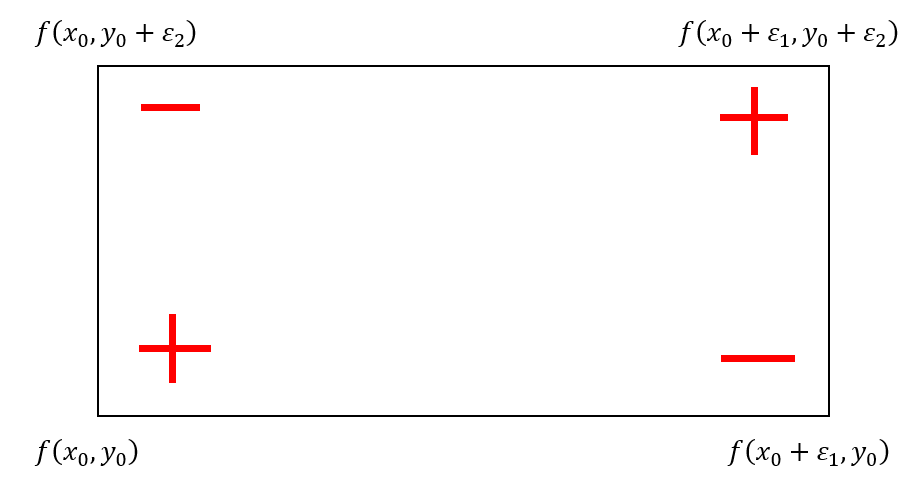
\includegraphics[scale=.35]{image1.png}}

    \begin{remark}
        Далее используются обозначения
        $f''_{xy}:=\frac{\delta^2 f}{\delta y \delta x}$,
        $f''_{yx}:=\frac{\delta^2 f}{\delta x \delta y}$
    \end{remark}

    \[\phi(\varepsilon_1, \varepsilon_2) =
        f(x_0, y_0)+f(x_0+\varepsilon_1, y_0+\varepsilon_2)
        -f(x_0+\varepsilon_1, y_0)-f(x_0, y_0+\varepsilon_2)\]
    %
    \[F_1(x)=f(x,y_0+\varepsilon_2)-f(x,y_0)
        \Rightarrow \phi = F_1(x_0+\varepsilon_1)-F_1(x_0) = \varepsilon_1 F'_1(\xi_1)\]
    \[F'_1(\xi_1)=f'_x(\xi _1, y_0+\varepsilon_2)-f'_x(\xi_1,y_0)=
        \varepsilon_2 f''_{xy}(\xi_1, \xi_2)
        \Rightarrow \phi = \varepsilon_1 \varepsilon_2 f''_{xy}(\xi_1, \xi_2)\]
    %
    \[F_2(y)=f(x_0+\varepsilon_1,y)-f(x_0,y)
        \Rightarrow \phi = F_2(y_0+\varepsilon_2)-F_2(y_0) = \varepsilon_2 F'_2(\eta_2)\]
    \[F'_2(\eta_2)=f'_y(x_0+\varepsilon_1,\eta_2)-f'_y(x_0,\eta_2)=
        \varepsilon_1 f''_{yx}(\eta_1, \eta_2)
        \Rightarrow \phi = \varepsilon_1 \varepsilon_2 f''_{yx}(\eta_1, \eta_2)\]
    %
    \[\phi = \varepsilon_1 \varepsilon_2 f''_{xy}(\xi_1, \xi_2) = \varepsilon_1 \varepsilon_2 f''_{yx}(\eta _1, \eta _2) \]
    \[\xi_1,\eta_1 \in [x_0, x_0+\varepsilon_1], \xi_2,\eta_2 \in [y_0, y_0+\varepsilon_2]\]
    %
    При $(\varepsilon_1, \varepsilon_2) \to 0:$
    $\frac{\phi}{\varepsilon_1 \varepsilon_2} \to f''_{xy}(x_0, y_0) = f''_{yx}(x_0, y_0)$
\end{proof}

\begin{cons}
    Если частные производные $\frac{\delta^2 f}{\delta x_i \delta x_j}$ и $\frac{\delta^2 f}{\delta x_j \delta x_i}$ непрерывны в точке и определены в её окрестности, то и равны в ней.
\end{cons}

%15
\section{Формула Тейлора с остатком в форме Пеано.}


$f: \mathbb{R}^n \to \mathbb{R}$. Сведём всё к одномерному случаю, т.к. одномерную формулу Тейлора мы знаем,
$x\in \mathbb{R}^n$ - центр разложения в ряд Тейлора, $y\in \mathbb{R}^n, h=y-x$.\\
$[x,y]$ - отрезок, его можно параметризовать так: $x+t(y-x)=x+th, t\in [0,1]$.\\
$\varphi (t) = f(x+th)$, эту функцию мы можем дифференцировать, т.к. это композиция дифференцируемых функций.\\
$\varphi' (t) = \langle \textrm{grad } f, h \rangle = \sum\limits_{k=1}^{n} \frac{\delta f}{\delta x_k} (x+th) h_k $\\
...\\
$\varphi^{(s)} (t) = \sum\limits_{1 \leq k_1,...,k_s \leq n}^{} \frac{\delta^s f}{\delta x_{k_1} ... \delta x_{k_s}} (x+th) h_{k_1}...h_{k_s} = \left(\left(\sum\limits_{k=1}^{n} \frac{\delta}{\delta x_k} h_k\right)^s f\right) (x+th)$\\
(последнее равенство следует воспринимать как удобное обозначение)
\[\varphi(\tau)=\sum\limits_{s=0}^{m} \frac{\varphi^s(0)}{s!}\tau^s + \underbrace{\frac{\varphi^{(m+1)}(\xi)}{(m+1)!}\tau^{(m+1)}}_{R_m(\tau,\varphi)}, \ \  \xi \in [0, \tau] \]
\[R_m(\tau,\varphi) = \int_{0}^{\tau} \frac{\varphi^{(m+1)}(l)}{m!}(\tau^{m}-l)^m dl = \int_{0}^{1} \frac{\varphi^{(m+1)}(l\tau)}{m!} \tau^{m+1} (1-l)^m dl \]
Подставим $\tau=1, t=0$, получим
\begin{stat}
    \add{taylor}{Формула Тейлора} с остатком в форме Пеано, $h=y-x$
    \[
        f(y) = \sum\limits_{s=0}^{m} \left(\left(\sum\limits_{k=1}^{n} \frac{\delta}{\delta x_k} h_k\right)^s \frac{f}{s!} \right) (x) + o(|h|^m)
    \]
\end{stat}

%16
\section{Формула Тейлора с остатком в интегральной форме.}


\begin{stat}
    Формула Тейлора с остатком в интегральной форме (см. прошлый билет), $h=y-x$
    \[
        f(y) = \sum\limits_{s=0}^{m} \left(\left(\sum\limits_{k=1}^{n} \frac{\delta}{\delta x_k} h_k\right)^s \frac{f}{s!} \right) (x) + \int_{0}^{1} \frac{(1-l)^m}{m!} \left(\left(\sum\limits_{k=1}^{n} \frac{\delta}{\delta x_k} h_k\right)^{m+1} f \right) (x+lh) dl
    \]
\end{stat}

%17 какой-то маленький билет
\section{Необходимое условие экстремума функции многих переменных.}


\begin{theorem}(\add{necextr}{Необходимое условие экстремума})
    $f: G\subset \mathbb{R}^n \to \mathbb{R}$ ($G$ открытое) гладкая, $x^0$ - точка локального минимума или максимума.
    Тогда $\textrm{grad } f\big|_{x^0} = 0$
\end{theorem}

\begin{proof}
    $\textrm{grad } f = \left(\frac{\delta f}{\delta x_1}, \frac{\delta f}{\delta x_2}, ... , \frac{\delta f}{\delta x_n} \right)$\\
    Пусть $\frac{\delta f}{\delta x_k}\big|_{x^0} \not= 0$, тогда
    $f(x^0_1, ..., x^0_{k-1}, x_k, x^0_{k+1}, ... , x^0_n) - f(x^0_1, ... ,x^0_n) = $\\
    $\underbrace{\frac{\delta f}{\delta x_k}\big|_{x^0}}_{\not=0}(x_k-x^0_k) +o(|x_k-x^0_k|)$
    $\Rightarrow \rightarrow\leftarrow$ (свелось к одномерному случаю)
    \begin{remind}
        Одномерный случай, $g: \mathbb{R} \to \mathbb{R}$ \\
        $g(x)=g(x^0)+g'(x^0)(x-x^0)+o(|x-x^0|)$
        \begin{enumerate}
            \item $g'(x^0)>0$, тогда при достаточно малом 
            $|x-x^0|: \\ 0 < g'(x^0)-\varepsilon< \frac{g(x)-g(x^0)}{x-x^0} < g'(x^0)+\varepsilon$,
            в таких окрестностях $g(x)>g(x^0)$ при $x>x^0$, $g(x)<g(x^0)$ при $x<x^0$, значит $x^0$ - не экстремум.
            \item $g'(x^0)<0$, тогда при достаточно малом 
            $|x-x^0|: \\ g'(x^0)-\varepsilon< \frac{g(x)-g(x^0)}{x-x^0} < g'(x^0)+\varepsilon < 0$,
            в таких окрестностях $g(x)<g(x^0)$ при $x>x^0$, $g(x)>g(x^0)$ при $x<x^0$, значит $x^0$ - не экстремум.
        \end{enumerate}
    \end{remind}
\end{proof}

%18 доказательство?
\section{Знак квадратичной формы. Достаточные условия экстремума функции многих переменных.}

\begin{defn}
    \add{sqform}{Квадратичная форма} $Q(x), x=(x_1, ..., x_n)$ - 
    это выражение вида $\sum\limits_{1 \leq k,l \leq n} a_{k,l} x_k x_l$, где $a_{k,l}$ - скаляр.  
\end{defn}

\begin{defn}
    (\add{signform}{Знак квадратичной формы})
    Квадратичная форма $Q(x), x\in \mathbb{R}^n, a_{k,l} \in \mathbb{R}$ положительно (отрицательно) определена, если для всех ненулевых $x: Q(x)>0 (Q(x)<0)$
    и знакопеременна, если может принимать как положительные, так и отрицательные значения.
\end{defn}

\begin{remark} (Квадр. форма на сфере)
    Легко видеть, что $Q(cx)=c^2 Q(x)$, где $c$ - скаляр, поэтому $Q(x)$ имеет тот же знак, что и $Q(cx)$,
    т.е. вдоль фиксированного направления кв. форма имеет фиксированный знак, а значит достаточно 
    рассматривать $x$ на сфере, чтобы определить знак кв.формы. Сфера - компакт, $Q(x)$ - непрерывная функция, 
    а потому $Q(x)$ достигает минимума и максимума на сфере. Тогда можно составить равносильное определение
    знака, квадратичная форма называется:
    \begin{itemize}
        \item положительно-определенной, если $ \displaystyle \min_{||x||=1} Q(x) > 0$
        \item отрицательно-определенной, если $ \displaystyle \max_{||x||=1} Q(x) < 0$
        \item знакопеременной, если $ \displaystyle \min_{||x||=1} Q(x) < 0 < \max_{||x||=1} Q(x)$
    \end{itemize}
\end{remark}

\begin{theorem}(\add{suffextr}{Достаточное условие экстремума})
    Пусть у $f: \mathbb{R}^n \to \mathbb{R}$ в точке $x^0$ нулевой градиент и определены все смешанные производные второго порядка.
    Тогда если квадратичная форма
    $Q(h)=\sum\limits_{1 \leq k,l \leq n} \frac{\delta^2 f}{\delta x_k \delta x_l}(x^0) h_k h_l$
    \begin{enumerate}
        \item положительно определена, значит $x^0$ точка локального минимума.
        \item отрицательно определена, значит $x^0$ точка локального максимума.
    \end{enumerate}
\end{theorem}

\begin{proof}
    Докажем для полож. квадр. формы, \hlink{taylor}{формула Тейлора}
    \[
        f(x) = f(x^0) + \frac{1}{2} \sum\limits_{1 \leq k,l \leq n} \frac{\delta^2 f}{\delta x_k \delta x_l} (x^0) (x_k-x_k^0) (x_l-x_l^0) + o(||x-x_0||^2)
    \]
    Обозначим $a_{k,l} = \frac{1}{2} \frac{\delta^2 f}{\delta x_k \delta x_l} (x^0)$\\
    При $x\not=x^0: \sum\limits_{1 < k,l\leq n} a_{k,l} (x_k-x_k^0) (x_l-x_l^0) = \langle A(x-x^0), (x-x^0) \rangle = Q(x-x^0) > 0$
    $\Rightarrow \exists \varepsilon>0: \ Q(x-x^0) \geq \varepsilon ||x-x^0||^2$

    \textit{Пояснение: } $Q(x)$ - положительная квадратичная форма, а потому 
    $\displaystyle \varepsilon = \min_{||x||=1} Q(x) > 0$,
    тогда $Q(x)=Q(||x||e)=Q(e)||x||^2 \geq \varepsilon ||x||^2$, т.к. $||e||=1$.

    Поделим равенство
    \[
        f(x) - f(x^0) = Q(x-x^0) + o(||x-x_0||^2)
    \]
    на $||x-x^0||^2$, тогда, если $||x-x^0||$ достаточно мало, то правая часть строго положительна.
\end{proof}

\begin{remark}
    Квадратичную форму можно привести к симметричному виду $\sum a_{k,l} h_k h_l$,  $a_{k,l}=a_{l,k}$,
    значит её можно привести и к диагольному виду $Q(h) = \sum_{k=1}^n \lambda_k h_k^2$
    \begin{itemize}
        \item $Q(h)$ положительна $\Leftrightarrow$ все $\lambda_k > 0$ ($x^0$ т. мин.)
        \item $Q(h)$ отрицательна $\Leftrightarrow$ все $\lambda_k < 0$ ($x^0$ т. макс.)
        \item $Q(h)$ знакопеременна $\Leftrightarrow$ $\exists k,l: \lambda_k < 0 < \lambda_l$ ($x^0$ не т. экстр.)
        \item иначе требуется дополнительное исследование
    \end{itemize}
\end{remark}

\begin{remark}
    Почему, если кв. форма знакопеременна, то $x^0$ не экстремум? Зафиксируем $y_1, y_2$ т.ч. $Q(y_1) < 0 < Q(y_2)$ и $||y_1||=||y_2||=1$.
    Тогда в равенство
    \[
        f(x) - f(x^0) = Q(x-x^0) + o(||x-x_0||^2)
    \]
    можно подставлять точки вида $x=cy_1+x^0$ ($\Rightarrow Q(x-x^0)=c^2 Q(y_1)$), в этом случае при достаточно малом $|c|=||x-x^0||$
    правая часть строго отрицательна; если же подставлять $x=cy_2+x^0$ - строго положительна.
\end{remark}

\begin{stat}
    \add{silvester}{Критерий Сильвестра} для симметричной квадратичной формы:
    \begin{enumerate}
        \item для положительной определённости квадратичной формы необходимо и достаточно, чтобы \href{https://ru.wikipedia.org/wiki/%D0%9C%D0%B8%D0%BD%D0%BE%D1%80_(%D0%BB%D0%B8%D0%BD%D0%B5%D0%B9%D0%BD%D0%B0%D1%8F_%D0%B0%D0%BB%D0%B3%D0%B5%D0%B1%D1%80%D0%B0)}
        {угловые миноры} её матрицы были положительны.
        \item Для отрицательной определённости квадратичной формы необходимо и достаточно, чтобы \href{https://ru.wikipedia.org/wiki/%D0%9C%D0%B8%D0%BD%D0%BE%D1%80_(%D0%BB%D0%B8%D0%BD%D0%B5%D0%B9%D0%BD%D0%B0%D1%8F_%D0%B0%D0%BB%D0%B3%D0%B5%D0%B1%D1%80%D0%B0)}
        {угловые миноры} чётного порядка её матрицы были положительны, а нечётного порядка — отрицательны.
    \end{enumerate}
\end{stat}

%19
\section{Касательные вектора. Касательная плоскость.}


\begin{stat}
    Есть уравнение $z=f(x,y)$ задающее плоскость и у $f$ есть частные производные в 
    $(x_0, y_0)$. 
    Тогда $z=f(x_0,y_0)$
    $+\df{f}{x}\big|_{(x_0,y_0)}(x-x_0)$
    $+\df{f}{y}\big|_{(x_0,y_0)}(y-y_0)$ - уравнение касательной плоскости.
    $(\frac{\delta f}{\delta x}\big|_{(x_0,y_0)}, \frac{\delta f}{\delta y}\big|_{(x_0,y_0)}, -1)$ - вектор нормали к кас.плоскости.
\end{stat}
%20
\section{Теорема о неявной функции для двух переменных.}%20


Это про случай $\mathbb{R}^2 \to \mathbb{R}$


\begin{theorem}
    $F: G\to \mathbb{R} (G\subset \mathbb{R}^2 - $ открытое $)$
    \begin{enumerate}
        \item $F(x_0, y_0) = 0$
        \item $F \in C^1(G)$
        \item $F'y(x_0, y_0) \not= 0$
    \end{enumerate} 
    Тогда $\exists I_x, I_y: \ \ x_0\in I_x, y_0 \in I_y, I_x\times I_y \subset \mathbb{R}^2$\\
    и $f: I_x\times I_y \in \mathbb{R}$ такая, что 
    $$F(x,y)=0 \Leftrightarrow y=f(x)$$
    $$f\in C^1, f'(x)=-\frac{F'_x(x,f(x))}{F'_y(x,f(x))}$$
\end{theorem}

\begin{remark}
    (неформальное рассуждение, почему такая формула) Предположим, что $f$ существует и дифференцируема,
    $F(x,f(x))=0$ на всей области определения $f$, продифференцируем левую и правую часть по правилу композиции
    $F'_x(x,f(x))+F'_y(x,f(x)) f'(x)=0$.
\end{remark}

\begin{proof}
    Существование: пусть функция $g_x(y) = F(x,y)$, будем считать, что в малой окрестности $V_{(x_0,y_0)}: \ $ 
    $F'_y > 0$, тогда $g(y)$ - возрастающая. Тогда $\forall x \in V \exists ! y: \ F(x,y)=0$. \\
    Непрерывность: рассмотрите прямоугольник с разрезами (т.е. $g_x(y)$). Так как решения уравнения $F(x,y)=0$ образуют
    замкнутое множество, то из того, что $x \to a$ и $f(x) \not\to f(a)$, следует, что есть второй корень на линии $x=a$, а у 
    нас корни единственные. \\
    Гладкость: $F(x+h,f(x+h))-F(x,f(x))=F(x+h,f(x)+(f(x+h)-f(x)))-F(x,f(x))=(F)$, при $h\to 0$ можно применять формулу Тейлора 
    для $F$, получим $(F)=h(F'_x(x,f(x))+\frac{f(x+h)-f(x)}{h}F'_y(x,f(x)))+o(|h|)$
\end{proof}


\section{Теорема о неявной функции для произвольного числа переменных.}%21


Это про случай $\mathbb{R}^m \to \mathbb{R}$


\section{Теорема о неявной функции для систем уравнений. Примеры.}%22

Это про случай $\mathbb{R}^{m+n} \to \mathbb{R}^n$
\begin{theorem}
    $x\in \mathbb{R}^m , y \in \mathbb{R}^n$\\
    $F: G\subset\mathbb{R}^{m+n}\to \mathbb{R}^n$
    \begin{itemize}
        \item $F\in C^1(G)$
        \item $F(x^0,y^0)=0$
        \item $F'_y(x^0,y^0)$ обратима (матрица $n\times n$ из частных производных)
    \end{itemize}
    тогда в некоторой окрестности $V_{(x^0,y^0)} \subset G$: 
    $$F(x,y) = 0 \Leftrightarrow y=f(x), \ f: V_{(x^0,y^0)} \to \mathbb{R}^n$$
    $$f'(x) = -(F'_y(x,f(x)))^{-1} F'_x(x,f(x))$$
\end{theorem}


\begin{proof}
    Докажем индукцией по $n$.\\
    \textit{База: } $n=1 \ \forall m$ доказано ранее.\\
    \textit{Переход: } $F=(F_1, F_2, ... , F_n), F_k: \mathbb{R}^{m+n} \to \mathbb{R}$.\\
    Имеем $n$ уравнений вида $F_k = 0$.\\ 
    \textit{Хотим: $y_k=f_k(x_1, x_2, ..., x_m)$, т.е. выразить каждый игрик через иксы.}\\
    Матрица невырождена, будем считать, что $\frac{\delta F_n}{\delta y_n} \not= 0$.\\
    Тогда $y_n = f^*(x_1, x_2, ... , x_m, y_1, ... , y_{n-1})$
    по предположению индукции. \\
    $\phi_k(x,y_1, ..., y_{n-1}) = F_k(x,y_1, ..., y_{n-1}, f^*), 1 \leq k \leq n-1$ ($\phi_n = 0$ из-за того, как выбрали $f^*$).
    $\frac{\delta \phi_k}{\delta y_l} = \frac{\delta F_k}{\delta y_l} + \frac{\delta F_k}{\delta y_n} \frac{\delta f^*}{\delta y_l}$\\
    Вспомним как выглядит невырожденная матрица $F'_y(x^0, y^0)$:
    $$
    \begin{pmatrix}
        \df{F_1}{y_1} & \df{F_1}{y_2} &\ldots & \df{F_1}{y_{n-1}} & \df{F_1}{y_n}\\
        \df{F_2}{y_1} & \df{F_2}{y_2} &\ldots & \df{F_2}{y_{n-1}} & \df{F_2}{y_n}\\
        \vdots                        & \vdots                        &\ddots & \vdots                        &  \vdots                      \\
        \df{F_{n-1}}{y_1} & \df{F_{n-1}}{y_2} &\ldots & \df{F_{n-1}}{y_{n-1}} & \df{F_{n-1}}{y_n}\\
        \df{F_n}{y_1} & \df{F_n}{y_2} &\ldots & \df{F_n}{y_{n-1}} & \df{F_n}{y_n}\\
    \end{pmatrix}    
    $$
    Добавим к первым $n-1$ столбцам последний, домноженный на скаляр, от этого матрица не перестанет быть невырожденной.
    $$
    \begin{pmatrix}
        \df{F_1}{y_1} + \df{F_1}{y_n} \df{f^*}{y_1} & \df{F_1}{y_2} + \df{F_1}{y_n} \df{f^*}{y_2} &\ldots & \df{F_1}{y_{n-1}} + \df{F_1}{y_n} \df{f^*}{y_{n-1}} & \df{F_1}{y_n}\\
        \df{F_2}{y_1} + \df{F_2}{y_n} \df{f^*}{y_1} & \df{F_2}{y_2} + \df{F_2}{y_n} \df{f^*}{y_2} &\ldots & \df{F_2}{y_{n-1}} + \df{F_2}{y_n} \df{f^*}{y_{n-1}} & \df{F_2}{y_n}\\
        \vdots                                      & \vdots                                      &\ddots & \vdots                                              & \vdots      \\
        \df{F_{n-1}}{y_1} + \df{F_2}{y_n} \df{f^*}{y_{n-1}}& \df{F_{n-1}}{y_2} + \df{F_{n-1}}{y_n} \df{f^*}{y_2} &\ldots & \df{F_{n-1}}{y_{n-1}}  + \df{F_{n-1}}{y_n} \df{f^*}{y_{n-1}} & \df{F_{n-1}}{y_n}\\
        \df{F_n}{y_1} + \df{F_n}{y_n} \df{f^*}{y_1} & \df{F_n}{y_2} + \df{F_n}{y_n} \df{f^*}{y_2} &\ldots & \df{F_n}{y_{n-1}} + \df{F_n}{y_n} \df{f^*}{y_{n-1}} & \df{F_n}{y_n}
    \end{pmatrix}  = 
    $$
    $$
    =
    \begin{pmatrix}
        \df{\phi_1}{y_1} & \df{\phi_1}{y_2} &\ldots & \df{\phi_1}{y_{n-1}} & \df{F_1}{y_n}\\
        \df{\phi_2}{y_1} & \df{\phi_2}{y_2} &\ldots & \df{\phi_2}{y_{n-1}} & \df{F_2}{y_n}\\
        \vdots           & \vdots           &\ddots & \vdots               &  \vdots \\
        \df{\phi_{n-1}}{y_1} & \df{\phi_{n-1}}{y_2} &\ldots & \df{\phi_{n-1}}{y_{n-1}} & \df{F_{n-1}}{y_n}\\
        \df{\phi_n}{y_1} & \df{\phi_n}{y_2} &\ldots & \df{\phi_n}{y_{n-1}} & \df{F_n}{y_n}\\
    \end{pmatrix} 
    =
    \begin{pmatrix}
          &   &        &   &   & \df{F_1}{y_n}    \\
          &   &        &   &   & \df{F_2}{y_n}    \\
          &   &\phi'_y &   &   & \vdots           \\
          &   &        &   &   & \df{F_{n-2}}{y_n}\\
          &   &        &   &   & \df{F_{n-1}}{y_n}\\
        0 & 0 & \ldots & 0 & 0 & \df{F_n}{y_n}
    \end{pmatrix} 
    $$
    откуда $det(\phi'_y) \df{F_n}{y_n} \not= 0 \Rightarrow det(\phi'_y) \not= 0$, а значит для системы $\{\phi_k\}_{k\leq n-1}=0$ применимо предположение индукции, т.е. $y_k = f_k(x)$ при $k \leq n-1$.
    Также получаем $y_n=f^*(x, f_1(x), ... , f_{n-1}(x))=f_n(x)$, что мы и хотели получить. Итоговая функция: $f(x)=(f_1(x), f_2(x), ... , f_n(x))$. Гладкость и искомая производная следуют из того, что мы умеем брать
    производную по композиции.  
\end{proof}



\section{Полярные и сферические координаты. Параметризации поверхностей.}%23


\section{Задача условного экстремума. Необходимое условие условного экстремума.}%24


\begin{stat}[Задача условного экстремума]
    Дана гладкая функция $f: G\subset\mathbb{R}^n \to \mathbb{R}$ и
    и соотношения между между переменными - уравнения(условия) с гладкими функциями 
    вида ($m \leq n$):
    \[
        \begin{cases}
            f_1(x_1, x_2, ... , x_n) = 0 \\
            f_2(x_1, x_2, ... , x_n) = 0 \\
            f_3(x_1, x_2, ... , x_n) = 0 \\
            \dots                        \\
            f_m(x_1, x_2, ... , x_n) = 0 
        \end{cases}  
    \]
    требуется найти условные экстремумы $f$.
\end{stat}

\begin{remark}
    В некоторых случаях можно $n-m$ переменных выбирать произвольно, остальные однозначно восстановятся.
\end{remark}

\begin{remark}
    $m$ соотношений задают какую-то поверхность, обозначим её $S$.
    %Будем считать, что $\dim S = n-m$.
    \textit{Все точки из S можно подставлять в $f$, можно вообще 
    считать, что $f_S: S \to \mathbb{R}$ и мы ищем экстремумы $f_S$}

    Зафиксируем точку $x^0 = (x^0_1, x^0_2, ... , x^0_n) \in S$. \\
    \textit{Хотим выяснить является ли она экстремальной.}

    Уравнение $f(x)=f(x^0)$ задаёт поверхность уровня, 
    обозначим её $L$. \\
    \textit{А вообще - это неважно.}

    Попробуем свести всё к одномерному случаю, для
    этого рассмотрим всевозможные гладкие кривые на $S$, проходящие через $x^0$, 
    т.е. гладкие функции вида 
    $x(t), t\in (-a, a), a \in \mathbb{R}_+, x(t) \in S$,
    $x(0)=x^0$. 
    
    Тогда вдоль такой кривой можно рассмотреть $h(t): t \mapsto f(x(t))$\\
    ($h: \mathbb{R} \to \mathbb{R}$), если т. $x^0$ условный экстремум $f$, 
    то $t=0$ экстр. для $h$ \\
    \textit{Пояснение:} иначе вдоль этой кривой из любой 
    окрестности т. $x^0$ можно пойти по $S$ так, чтобы $f$ возрастала; и так, чтобы
    убывала; пойти = сдвинуть значение $t$ ($t$ - это просто число); оставаясь
    на $S$ мы соблюдаем все $m$ условий, так что всё корректно.\\
    %
    Тогда необходимо, чтобы $h'(0)=0$. По правилу композиции: 
    $h'(0)=(f(x(t)))'\big|_{0}=\sum\limits_{k=1}^{n} \df{f}{x_k}(x(0)) \df{x_k}{t}(0)=$
    $\sum\limits_{k=1}^{n} \df{f}{x_k}(x^0) \df{x_k}{t}(0)=\langle \textrm{grad } f(x(0)), x'(0) \rangle = 0$.
    
    \begin{remind}[geometry reference]
        Два вектора называются перпендикулярными, если их 
        скалярное произведение равно нулю. 
    \end{remind}

    \textit{Что это значит? Если говорить о каком-то геометрическом смысле, 
    то мы получили следующее утверждение: скалярное произведение нуль, значит
    градиент $f$ в т. $x^0$ перпендикулярен касательному вектору $S$ в т. $x^0$ 
    (почему $x'(0)$ это касательный вектор? Да потому что он сам по себе градиент,
    т.е. состоит из производных. В данном случае $x(t)$ это кривая, так что
    и касательный вектор, подразумевается, соответствующий этой кривой)}
    
    Рассматривая всевозможные кривые $x(t)$ можно получать 
    касательный вектор $x'(0)$ по любому направлению в касательной плоскости.
    \textit{Пояснение-цитата от Белова:} ну и понятно, что если мы посмотрим 
    все гладкие кривые на поверхности $S$, проходящие через точку $x^0$, 
    то в качестве касательных векторов мы получим любой вектор из касательной 
    плоскости.

    Но тогда мы получаем вывод, что градиент $f$ в т. $x^0$ 
    перпендикулярен любому вектору из касательной плоскости, т.е. перпендикулярен
    всей касательной плоскости к $S$ в т. $x^0$ \textit{(это тавтология по сути)}\\
    \textit{Равносильное утверждение: у $S$ и $L$ совпадают кас. плоскости в т. $x^0$;
    равносильность следует из того, что градиент всегда перпендикулярен касательной плоскости}

    Градиенты $f_k$-ых тоже перпендикулярны касательной плоскости к $S$. 

    $\Rightarrow f \in Lin(f_k)$, т.е. $f=\sum\limits_{k=1}^{m} \lambda_k f_k$
\end{remark}



\section{Функции Лагранжа. Достаточное условие условного экстремума. Примеры.}%25

\hindex{flagrange}{Функция Лагранжа}
\begin{defn}
    Пусть есть $m$ условий вида $F_k(x_1, ... , x_n) = 0$ и мы хотим найти условный 
    экстремум $F(x_1, ... , x_n)$. Рассмотрим \htarg{flagrange}{функцию Лагранжа} 
    $L(x_1, ... x_n, \lambda_1, ..., \lambda_m)=F-\sum\limits_{k=1}^{m} \lambda_k F_k$,
    тогда все частные производные $L$ должны быть нулевыми. 
\end{defn}



\section{Теорема о перестановке пределов. Общий вид теоремы Стокса-Зайделя.}%26


\section{Голоморфные функции. Примеры. Общий вид дифференциала голоморфной функции.}%27


\section{Степенные ряды. Радиус сходимости степенного ряда.}%28


\section{Голоморфность суммы степенного ряда.}%29


\section{Теорема Стоуна-Вейерштрасса. Лемма об аппроксимации |x|.}%30


\begin{remark}
    $d(f,g) = \sup|f-g|$
\end{remark}

\begin{remark}
    $K$ - компактное множество. $C(K)$ - пространство непрерывных функций на нём.
\end{remark}

\begin{defn}
    $\mathcal{A}$ - \add{algebra}{Алгебра в пространстве непрерывных функций},
    если $\mathcal{A} \subset C(K)$ и $\mathcal{A}$ - линейное векторное 
    пространство такое, что $f,g \in \mathcal{A} \Rightarrow fg \in \mathcal{A}$.
\end{defn}

\hindex{points}{Выделение/разделение точек}
\begin{defn}
    $\mathcal{A}$ \htarg{points}{выделяет} точки, если
    $\forall x \in K \exists f \in \mathcal{A}: \ f(x)\not=0$\\
    $\mathcal{A}$ \htarg{points}{разделяет} точки, если
    $\forall x_1, x_2 \in K \exists f \in \mathcal{A}: \ f(x_1)\not=f(x_2)$
\end{defn}

\begin{theorem}
    $\mathcal{A}$ - алгебра, $\mathcal{A} \subset C(K)$, $K$ - компактно и хаусдорфово,
    $\mathcal{A}$ выделяет и разделяет точки. Тогда $\overline{\mathcal{A}}=C(K)$.
\end{theorem}

%31
\section{Теорема Стоуна-Вейерштрасса. Завершение докзательства.}

%32
\section{Теорема о неподвижной точке. Приложение к дифференциальным уравнениям.}


\begin{defn}
    \add{contrmap}{Сжимающее отображение} $T: X \to X$, $X$ - полное метрическое пространство с метрикой $\rho$
    $$\exists \alpha < 1: \ \rho(Tx, Ty) \leq \alpha \rho (x,y)$$ 
\end{defn}

\begin{theorem}
    У сжимающего отображения $T$ есть единственная неподвижная точка, т.е. такая, что $Tx=x$. 
\end{theorem}

\begin{proof}
    \textit{Единственность:} пусть $x$ и $y$ - две неподвижные точки отображения $T$, тогда 
    $\rho (x,y) = \rho (T x, T y) \leq \alpha \rho (x,y)$, откуда $1 \leq \alpha$, противоречие. \\
    \textit{Существование:} расммотрим орбиту $x$, т.е. $x, Tx, T(Tx)=T^2 x, ... , T^n x, ...$, такая последовательность фундаментальна:
    $$\forall \varepsilon > 0 \ \exists N \ \forall n,m > N: \ \rho (T^n x, T^m x) < \varepsilon $$
    действительно, при $n \leq m:$ 
    $\rho (T^n x, T^m y) \leq \alpha^n \rho (x, T^{m-n} x) \leq $  
    $\alpha^n \sum\limits_{k=0}^{\infty} \rho (T^k x, T^{k+1} x) \\$ 
    $\leq \alpha^n \sum\limits_{k=0}^{\infty} \alpha^k \rho (x, Tx) = $
    $\frac{\alpha^n \rho (x,Tx)}{1-\alpha}  < \varepsilon$. 
    А значит $\exists \lim\limits_{n \to \infty} T^n x = e \in X$ - неподвижная точка, 
    т.к. $T^n x \to e \Rightarrow T(T^n x) = T^{n+1} x \to Te = e$ (суть в том, что $Te$ отличается от $T^{n+1}e$ на сколь угодно мало,
    а значит $Te = \lim\limits_{n+1 \to \infty} T^{n+1} x = e$).  
\end{proof}

\begin{remark}
    $\rho(T^n x, T^m y) < \varepsilon$ при $n,m>N$.
\end{remark}
%33
\section{Топология в пространстве бексконечно дифференцируемых над R функций. Метризуемость.}

\begin{remark}
    Сходимость: будем говорить, что последовательность
    $\{f_j\}_{j\in\mathbb{N}} \subset C^\infty(R)$ сходится к $f \in C^\infty(R)$, 
    если для любого компактного множества $K \subset R$ функции $f_j$
    сходятся к $f$ равномерно на $K$.
\end{remark}

\begin{stat}
    $$
    d(f,g) = \sum\limits_{j,n\geq 0} \frac{ ||f^{(j)}-g^{(j)}||_{\infty,I_n}}
    {1+||f^{(j)}-g^{(j)}||_{\infty, I_n}} 2^{-j-n}
    $$
    ($I_n$ - компакты, $||\cdot||_\infty = \sup||\cdot||$) тогда $d$ - метрика.
\end{stat}

\begin{stat}
    Топология порожденная такой метрикой и топология порожденная такой сходимостью совпадают.
\end{stat}

\newpage
\hypertarget{t2}{}
\printindex


\end{document}
